% !TeX spellcheck = da_DK
% Setup document class.
%  This will always be the beamer class, but depending on the use of notes,
%  it can be annotated with the option [notes] or  [notes=only], depending
%  on whether notes should be included, or should be the only thing in
%  the document.
\documentclass{beamer}

% Setup theme.
%\usetheme[
%%% options passed to the outer theme
%    progressstyle=fixedCircCnt,   %either fixedCircCnt, movCircCnt, or corner
%    rotationcw,          % change the rotation direction from counter-clockwise to clockwise
%    shownavsym          % show the navigation symbols
]{AAUsimple}

\usetheme[
%%% options passed to the outer theme
%    hidetitle,           % hide the (short) title in the sidebar
%    hideauthor,          % hide the (short) author in the sidebar
%    hideinstitute,       % hide the (short) institute in the bottom of the sidebar
%    shownavsym,          % show the navigation symbols
%    width=2cm,           % width of the sidebar (default is 2 cm)
    hideothersubsections,% hide all subsections but the subsections in the current section
%    hideallsubsections,  % hide all subsections
    left               % right of left position of sidebar (default is right)
%%% options passed to the color theme
%    lightheaderbg,       % use a light header background
  ]{AAUsidebar}



% Import preamble
%%% Initial things %%%
% Increase number of dimen registers
\usepackage{etex}
% Fix various issues with LaTeX2e
\usepackage{fixltx2e}
% Font package
\usepackage{fourier}


%%% Translations and character encodings %%%
% Enable use of several characters, including æ, ø and å
\usepackage[utf8]{inputenc}
% Danish language
\usepackage[danish]{babel}
% Use PostScript fonts instead of bitmap ones. Also does other stuff.
\usepackage[T1]{fontenc}
% Various LaTeX symbols
\usepackage{latexsym}
% Wider selection of colours
\usepackage{xcolor}
% Improved element justification
\usepackage{ragged2e}
% Font improvements
\usepackage{fix-cm}
% Enables various forms of lines, like double-underlining (\uuline{})
\usepackage{ulem}
% Sets the tolerance for distance between words, determining when to hyphenate.
\pretolerance=2500


%%% Figures and tables (Floats) %%%
% Enable multi-rows and -columns
\usepackage{multirow}
\usepackage{multicol}
% Double, horizontal lines
\usepackage{hhline}
% Enables coloured tables
\usepackage{colortbl}
% Prettier tables
\usepackage{booktabs}


%%% Mathematic formulas %%%
% AMS math
\usepackage{amsmath}
\usepackage{amssymb}
% Extra fonts (for math, I think)
\usepackage{stmaryrd}
% Access text symbols
\usepackage{textcomp}
% Extend AMS
\usepackage{mathtools}
\usepackage{cancel}


%%% Graphics %%%
% Various image-commands
\usepackage{eso-pic}
% Use JPEG and PNG images
\usepackage{graphicx}


%%% References, bibtex and URLs %%%
% Post URLs. Allows breaking at hyphens to help avoid long links.
\usepackage{url}
% Better cross references
\usepackage[danish]{varioref}
% Define a new 'leo' style for URL package, that will use a smaller font
\makeatletter
\def\url@leostyle{%
  \@ifundefined{selectfont}{\def\UrlFont{\sf}}{\def\UrlFont{\small\ttfamily}}
}
\makeatother
% And of course, use this new style
\urlstyle{leo}

\hypersetup{pdfstartview={Fit}}

% Define document stuff
\title[Sejlklubadministration]{Bådudlån i sejlklubber}
\subtitle[Statusseminar]{Statusseminar}
\author[SW2A305]{Gruppe SW2A305}
\date{10. marts 2014}

\institute[
%  {\includegraphics[scale=0.2]{aau_segl}}\\ %insert a company, department or university logo
Første Studieår (Software)\\
Aalborg Universitet\\
Danmark
] % optional - is placed in the bottom of the sidebar on every slide
{% is placed on the title page
  Første Studieår --- Software\\
  Aalborg Universitet\\
  Danmark
  
  %there must be an empty line above this line - otherwise some unwanted space is added between the university and the country (I do not know why;( )
}

% Specify a logo on the titlepage (you can specify additional logos an include them in 
% institute command below
\pgfdeclareimage[height=1.5cm]{titlepagelogo}{AAUgraphics/aau_logo_new} % placed on the title page
%\pgfdeclareimage[height=1.5cm]{titlepagelogo2}{graphics/aau_logo_new} % placed on the title page
\titlegraphic{% is placed on the bottom of the title page
  \pgfuseimage{titlepagelogo}
  %  \hspace{1cm}\pgfuseimage{titlepagelogo2}
}


\begin{document}

{\aauwavesbg
  \begin{frame}[plain,noframenumbering]
    \titlepage
  \end{frame}}

% ==================== SUBJECTS ======================
%% !TeX spellcheck = da_DK
\section{Section 1}

% === Slide: Title ===
\begin{frame}{Title of frame}

\structure{This is part of the structure.}

\vspace{2mm}

This is some text\ldots

\note{This is a note}

\begin{itemize}
  \item First point
  \item Second point
\end{itemize}

\note{Another note here\ldots}

\end{frame}

% --- Subsection name ---
\subsection{Subsection 1}

% === Slide: Another title ===
\begin{frame}{Another title}

Wee!

\end{frame}

\section{Introduktion}

\begin{frame}{Introduktion}

	\framesubtitle{Introduktion af Projekt}

	\begin{itemize}
		\item Administration af skolebåde og bådudlån i en sejlklub
		\item Analyse organisering
			\begin{itemize}
				\item Generelt til specifikt - Mere om det ved Thomas
			\end{itemize}
		\item Blyant og papir bruges meget i sejlklubben
	\end{itemize}
	
\end{frame}
\section{Interessenter}
\begin{frame}{Interessenter}
	\framesubtitle{Analyse af interessenterne}
	
	\begin{itemize}
		\item Fritidsklubber
		\item Fodbold
		\item Badminton og tennis
		\item Skydning
		\item Golf
		\item Haller
		\item Netcaféer
		\item Sejlklubber
	\end{itemize}


\end{frame}

\section{Test}
\begin{frame}{Organisation}
	\framesubtitle{Analyse af organisationen}
		\begin{itemize}
			\item Interessenter for sejlklubbers administrative opgaver
			\begin{itemize}
				\item Dansk Sejlunion
				\item Medlemmer
				\item Undervisere
			\end{itemize}
			\item Research af klubber
			\begin{itemize}
				\item Sejlklubben Sundet
				\item Andre sejlklubber
			\end{itemize}
		\end{itemize}

\end{frame}

\section{Teknologi}

\begin{frame}{Teknologi}
  \framesubtitle{State of the Art}
  
  \begin{itemize}
    \item To systemer
    \begin{itemize}
      \item BoatCloud
      \item Sailing Club Manager
    \end{itemize}
    \item Få ligheder --- Mange forskelle
    \vspace{2mm}
    \item Managementsystemer
    \begin{itemize}
      \item Samling af processer og procedurer.
      \item Frivillige organisationer og virksomheder.
      \item Sailing Club Manager er et eksempel.
      \item Nikolaj vil vende tilbage til det\ldots
    \end{itemize}
  \end{itemize}
\end{frame}

\section{Problemformulering}

\begin{frame}{Problemformulering}
  
  \begin{itemize}
    \item Generelt problem
    
    \item Sejlklub specifikationer
    
    \item Management system
    
    \item Reducering af arbejdsbyrde
    
  \end{itemize}
\textit{Det er et problem at sejlklubben Sundet bruger unødige ressourcer på fysisk bogføring.
Kan der laves et system som kan håndtere alle de data som bliver bogført, nedsætter
recourceforbruget og samtidigt er nemt at bruge?}
\end{frame}

\section{Det videre forløb}

\begin{frame}{Det videre forløb}
\framesubtitle{Programmet}

	\begin{itemize}
	\item Brugerflade
		\begin{itemize}
		\item Laves ved hjælp Visual Studio
		\item Metode ikke besluttet endnu
		\item Web implementering 
		\end{itemize}
		
	\item Funktioner
		\begin{itemize}
		\item Båd booking
		\item Betaling
		\item Af-/tilmelding af undervisning
		\item Medlemshåndtering
		\end{itemize}	
		
	\end{itemize}

\end{frame}

\begin{frame}{Det videre forløb}
\framesubtitle{UML-diagram}

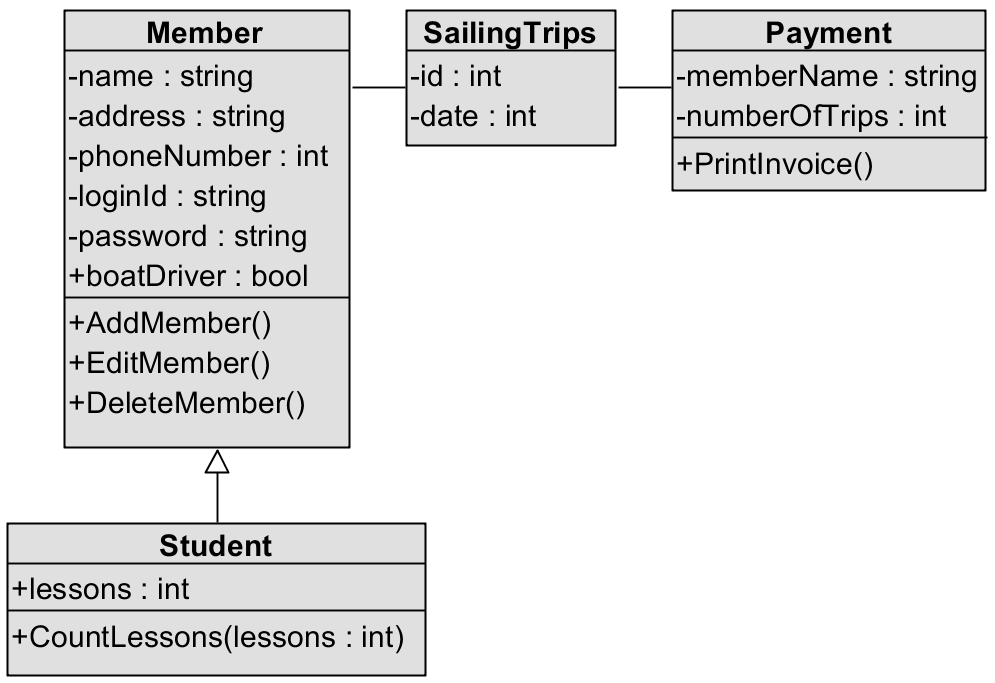
\includegraphics[width=0.8\textwidth,height=0.8\textheight,keepaspectratio]{images/UML-diagram.png}

\end{frame}
% ====================================================

% Final slide
{\aauwavesbg
  \begin{frame}[plain,noframenumbering]
    \finalpage{\texttt{\textbf{return} 0;}}
  \end{frame}}

\end{document}
